\chapter{总结与展望}
本章对本文的研究内容做一个总结。首先讨论GMSC与CountMax结合的可行性,随后介绍了本文解决的问题和未解决的问题。

\section{GMSC与CountMax的结合}

为了使得GMSC与sketch能够在现有的生产环境中应用,本节简要讨论GMSC在实际的SDN环境中实现的可行性。

GMSC的实现包括两个重要部分:其一是控制器与交换机之间的通信,其二是交换机上对数据包和掩码的匹配。
P4\cite{bosshart2014p4}是一种可以同时解决这两个问题的一揽子解决方案。
P4是一个用来描述数据包处理流程的高级语言,它可以理解为是OpenFlow协议的替代者,是一种可编程的SDN南向协议。
Juniper已于2018年2月表示将支持P4作为控制器与交换机间的可选协议\cite{juniper2018p4}。
在UnivMon\cite{liu2016one}的实现部分中,数据平面中的采样、sketch等处理就是使用P4实现的。

\begin{figure}[ht]
	\centering
	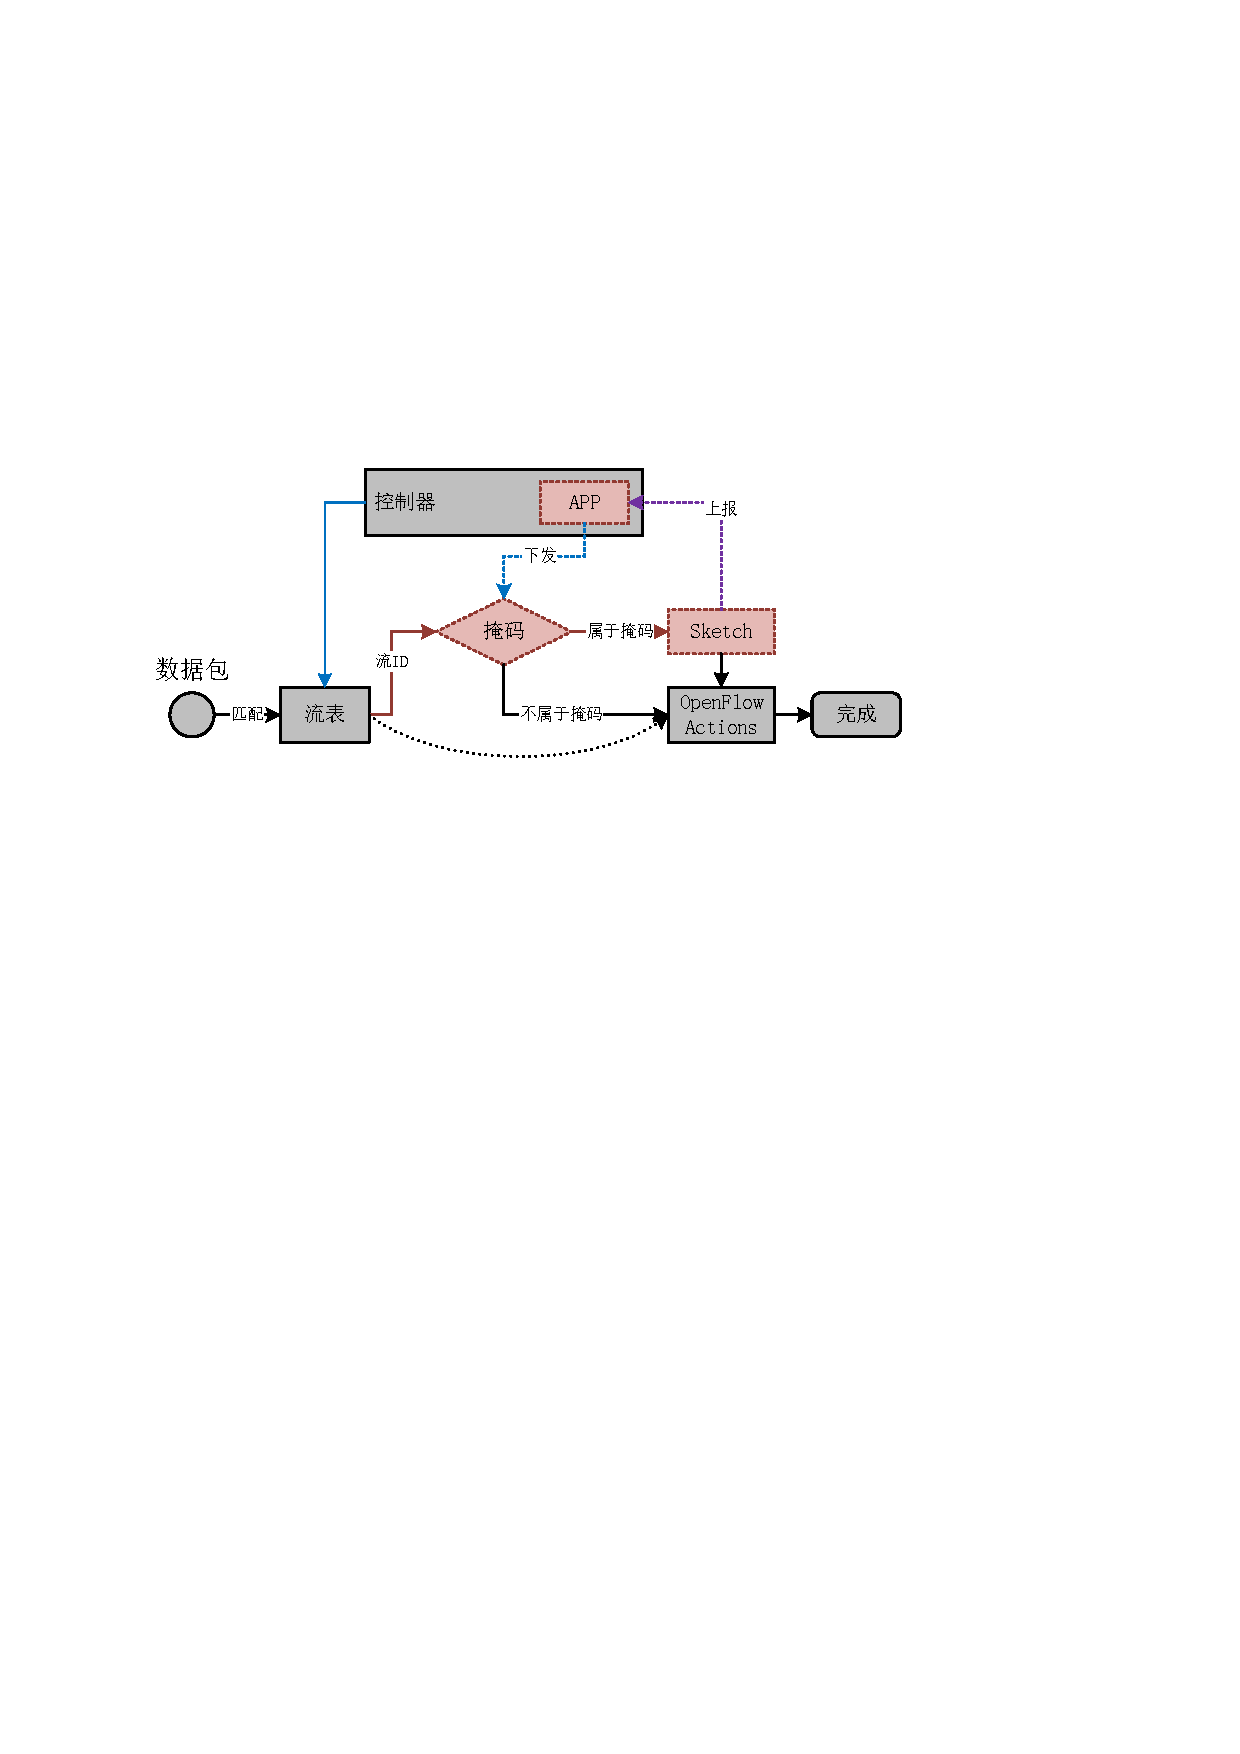
\includegraphics[width=0.75\textwidth]{fig/private.pdf}
	\caption{使用私有协议的实现方式}
	\label{fig:private}
\end{figure}

除P4方案外,对于可编程的交换机,我们还可以通过实现私有协议或者修改OpenFlow协议实现。
如UnivMon\cite{liu2016one}的作者提供的实现当中,控制器和交换机之间的通信就是通过私有的RPC(远程过程调用)管道实现的。
本文第\ref{sec:proto}节中,使用一个专门的TCP连接进行sketch数据的上报。
如使用私有协议,可以在sketch运行的第一步添加判断流ID是否属于激活的掩码的判断,从而实现数据包和掩码的匹配。

图\ref{fig:private}为本文基于OVS平台上的私有协议的实现。其中红色框体属于本文开发的内容。
如图所示,在控制平面中,sketch的控制APP寄宿在控制器中,通过独立的信道进行掩码的下发和流量统计数据的收集。
在数据平面中,所有的数据包在进行流表项匹配后,都会进行判断是否属于下发的掩码。
若属于,则交给sketch进行处理,随后再执行流表项中规定的操作。

修改OpenFlow协议的方法则是在正常的OpenFlow协议的基础上增加一种操作(Action),从而能够将“匹配掩码的数据包传输给sketch处理”的规则转换为流表直接发送到交换机。
在交换机上对这种自定义操作进行实现,使得它在被执行的时候会调用sketch处理此数据包。

\begin{figure}[ht]
	\centering
	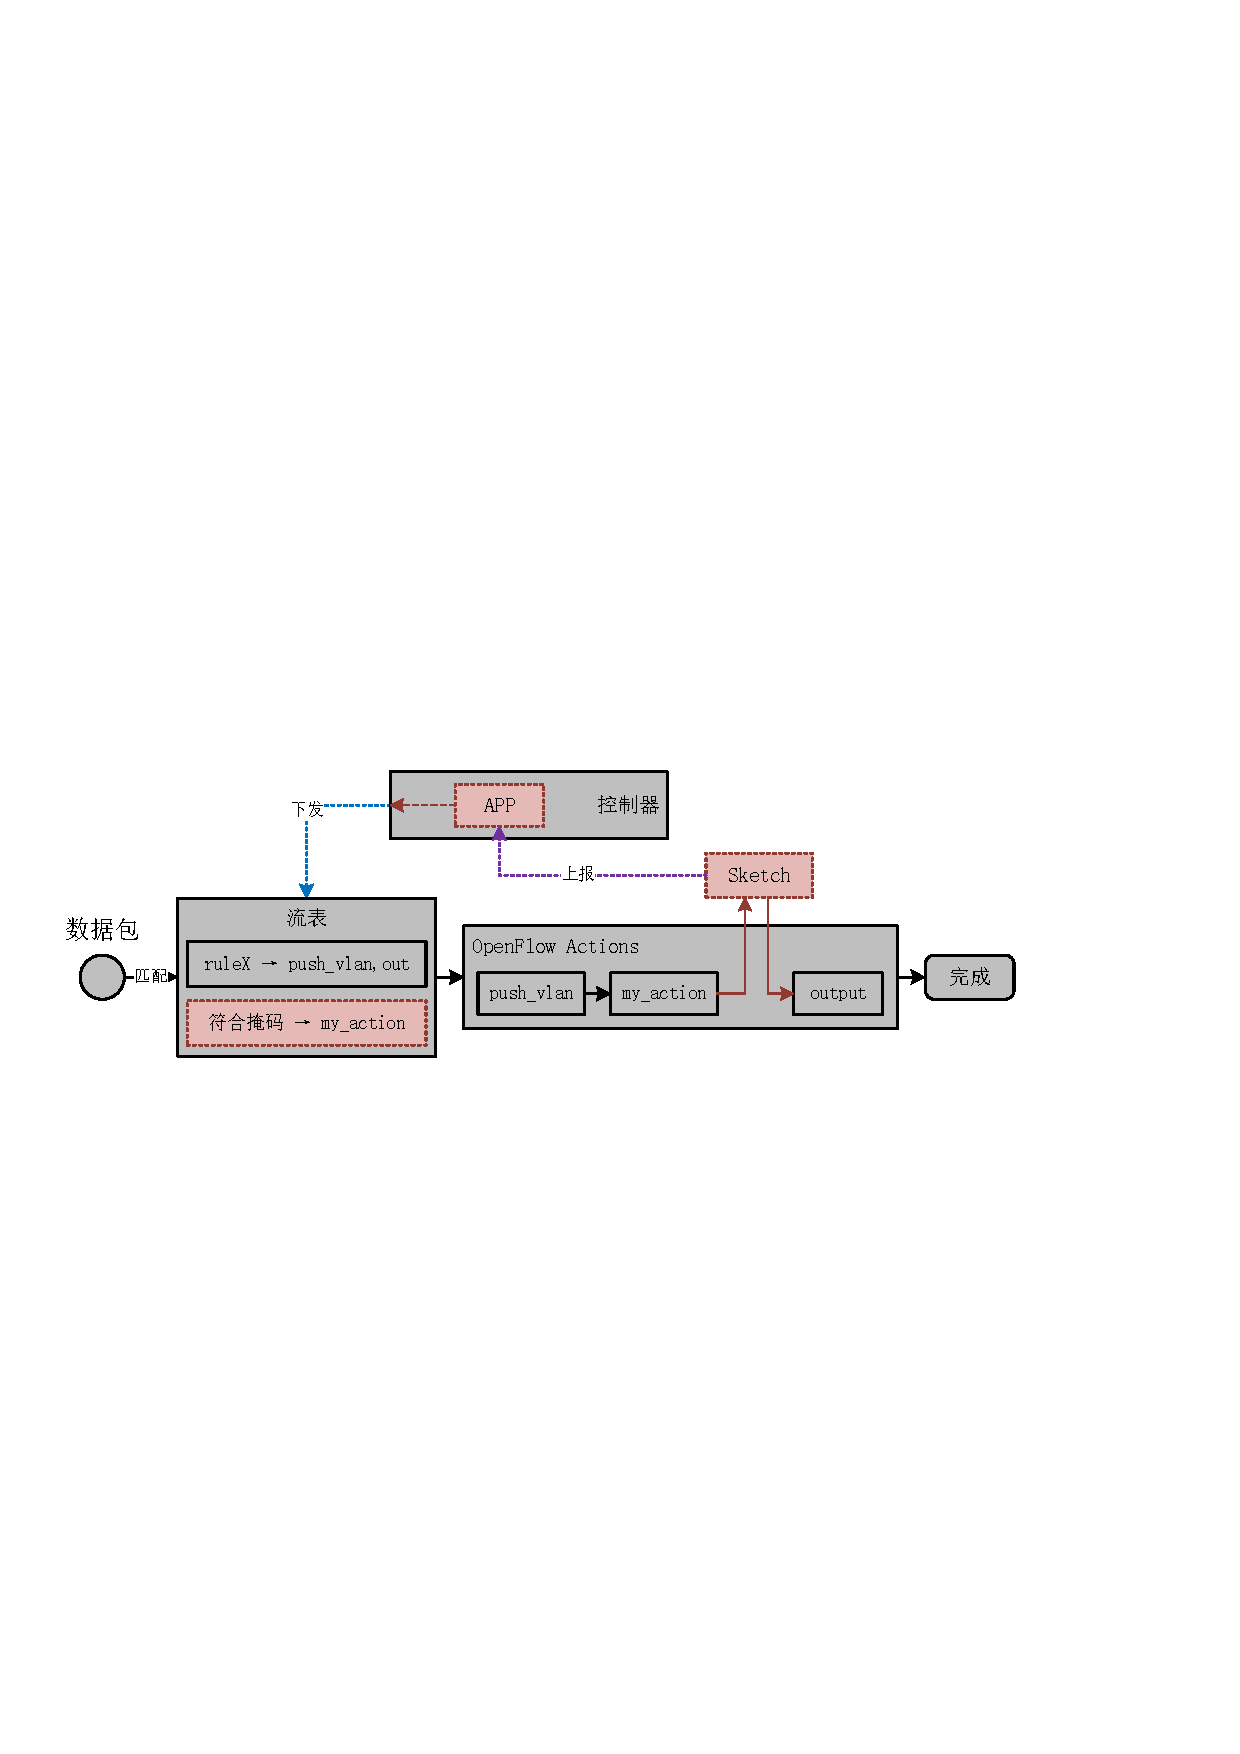
\includegraphics[width=\textwidth]{fig/ofaction.pdf}
	\caption{扩展OpenFlow的实现方式}
	\label{fig:ofaction}
\end{figure}

图\ref{fig:ofaction}为扩展OpenFlow协议实现方式的示意图。
首先编辑控制器和交换机上OpenFlow协议的实现,增加一个名为my\_action的操作,
并在交换机上将my\_action操作实现为调用sketch对数据包进行处理的操作。
控制APP通过控制器向交换机下发掩码的规则,指定匹配掩码的流要执行操作my\_action。
对于匹配的数据包,在交换机按照OpenFlow协议执行操作链时,my\_action会被执行,调用sketch进行统计,然后回到OpenFlow Action的管线中。

%本文实现了以下功能:私有协议下的控制APP和OVS组件,以及扩展了OpenFlow、可通过控制台输入自定义操作的OVS。

\section{论文解决的问题}
本文首先梳理了软件定义网络中流量测量的重要性、调研并介绍了若干种现有的测量方法和sketch,且提出了流量测量分布式部署的问题。
随后,本文提出了名为CountMax的sketch。和现有的sketch相比,CountMax处理数据包所需的计算资源降低了约三分之一,但精度丝毫不逊色。
通过仿真模拟和系统集成测试,我们得出结论,CountMax可以胜任流量测量的任务。
之后,通过对流量测量分布式部署的建模与分析,本文引出了最大化流统计覆盖(MSC)问题,并给出了解决此问题的算法GMSC。
仿真模拟显示,将GMSC和CountMax结合,可以在有效地均摊计算负载的同时,提高测量精度。
最后,本文讨论了GMSC+CountMax在实际系统中的实现方法。

\section{尚未解决的问题}
本文尚未解决的问题,以及未来的研究方向主要有两点。
第一点是GMSC算法非常依赖流的先验知识。
对sketch进行预先部署不可避免的要依赖于先验知识,尽可能地减少所需的先验知识是一个研究方向。
另外,如果能够开发出可以动态调节的部署方式,利用实时数据动态进行部署也是一个可行的方向。
第二点是GMSC+CountMax系统的完善实现。本文所实现的系统只是验证可行性的原型,要让系统变得能够实际应用,还需要庞大的工程。
若采用私有协议,则必须考虑协议未来升级的可能性,注重可扩展性和兼容性。
若选择扩展OpenFlow协议,由于不同设备有着不同的OpenFlow实现,需要进行大量的设备适配和兼容性测试。